\section{Analysis of Sink Tokens}
\label{sec:mechanisms}

The efficiency and performance improvements demonstrated by our Fast Nystr\"om Attention (Section~\ref{sec:fna}) method and masking-based denoising method (Section~\ref{sec:performance_efficiency}) stem from fundamental mechanisms governing token interactions in vision transformers. In particular, we identify \emph{mutual suppression} among tokens as the driving force behind the emergence of massive and artifact tokens. Below, we detail how this suppression shapes attention dynamics, underpins efficient approximations, and motivates our masking strategy.

\subsection{Mechanisms of Token Suppression}

Our experiments show that massive tokens emerge through a distinct \emph{phased} progression, driven by mutual suppression and magnified by MLP layers. Although the following layer indices refer specifically to CLIP ViT L-14, the same qualitative patterns arise in other pretrained ViTs.

\paragraph{Emergence Phase (Layers 9--10).}
In the early-to-mid layers (e.g., layers 9 and 10 in CLIP ViT L-14), tokens with slightly larger activations begin to exhibit suppressive behaviors toward other potential sink tokens (including themselves). These suppressive signals, when passed through the MLP’s nonlinear transformations, create a compounding feedback loop. Once a token has a slight size advantage, it increasingly dampens its competitors’ growth while growing itself. Concretely, in a multi-head self-attention block, each token $j$ (serving as a \emph{key}) contributes a rank-$H$ subspace
\begin{align}
    \Sl{\ell}_j = \text{span}(\cbn{\Vl{\ell}_{h, j}}_{h \in [H]}) \subspace \R^d
\end{align}
which influences other tokens (as \emph{queries}) via the weighted combination from attention. When a (potentially) massive token $j$ has a large norm, its subspace $\mathcal{S}_j^{(\ell)}$ tends to \emph{negatively} project onto other tokens in attention, yielding a \emph{destructive} or suppressive effect on their subsequent activations.
% \begin{align} \resizebox{\columnwidth}{!}{$
%     \attn{\ell}(\Embp{\ell})_i = \Olb{\ell} + \dss{j}{} \dss{h}{} \sf\pfrac{\Ql{\ell}_{h, i}{\mbf{K}^{(\ell)\top}_h}}{\sqrt{d'}}_j\Vl{\ell}_{h, j}{\mbf{O}^{(\ell)\top}_{h, weight}}.
% $}
% \end{align} 
% When a (potentially) massive token $j$ has a large norm, its subspace $\mathcal{S}_j^{(\ell)}$ tends to \emph{negatively} project onto other tokens in the MLP, yielding a \emph{destructive} or suppressive effect on their subsequent activations.

\paragraph{Consolidation Phase (Layers 11--12).} 
The largest tokens fully mature into massive tokens in layers 11 and 12, absorbing a disproportionately large share of attention from all other tokens. Since attention weights are nonnegative (post-softmax), the dominant tokens effectively channel attention values in a way that \emph{further} suppresses remaining mid-sized contenders. Mathematically, if $P_{i,j}$ measures the mean normalized projection of token $j$’s subspace onto $i$:
\begin{align}
    P_{i, j}
    = \frac{1}{H} \dss{h}{} \frac{\innern{\emb{\ell}{i}, \Vl{\ell}_{h, j}}}{\normn{\emb{\ell}{i}}}
    = \inner{\frac{\emb{\ell}{i}}{\normn{\emb{\ell}{i}}}, \frac{1}{H} \dss{h}{} \Vl{\ell}_{h, j}},
\end{align}
then a \emph{strongly negative} $P_{i,j}$ indicates $j$ significantly \emph{suppresses} $i$. In layers 9--10, the potential sink tokens heavily penalize each other’s growth; by layers 11--12, a small number of them have ``won'' the competition and become the new attention sinks as seen in Appendix \ref{sec:appendix_analysis} Figure \ref{fig:massive_token_evolution}.

\begin{figure*}[!t]
    \centering
    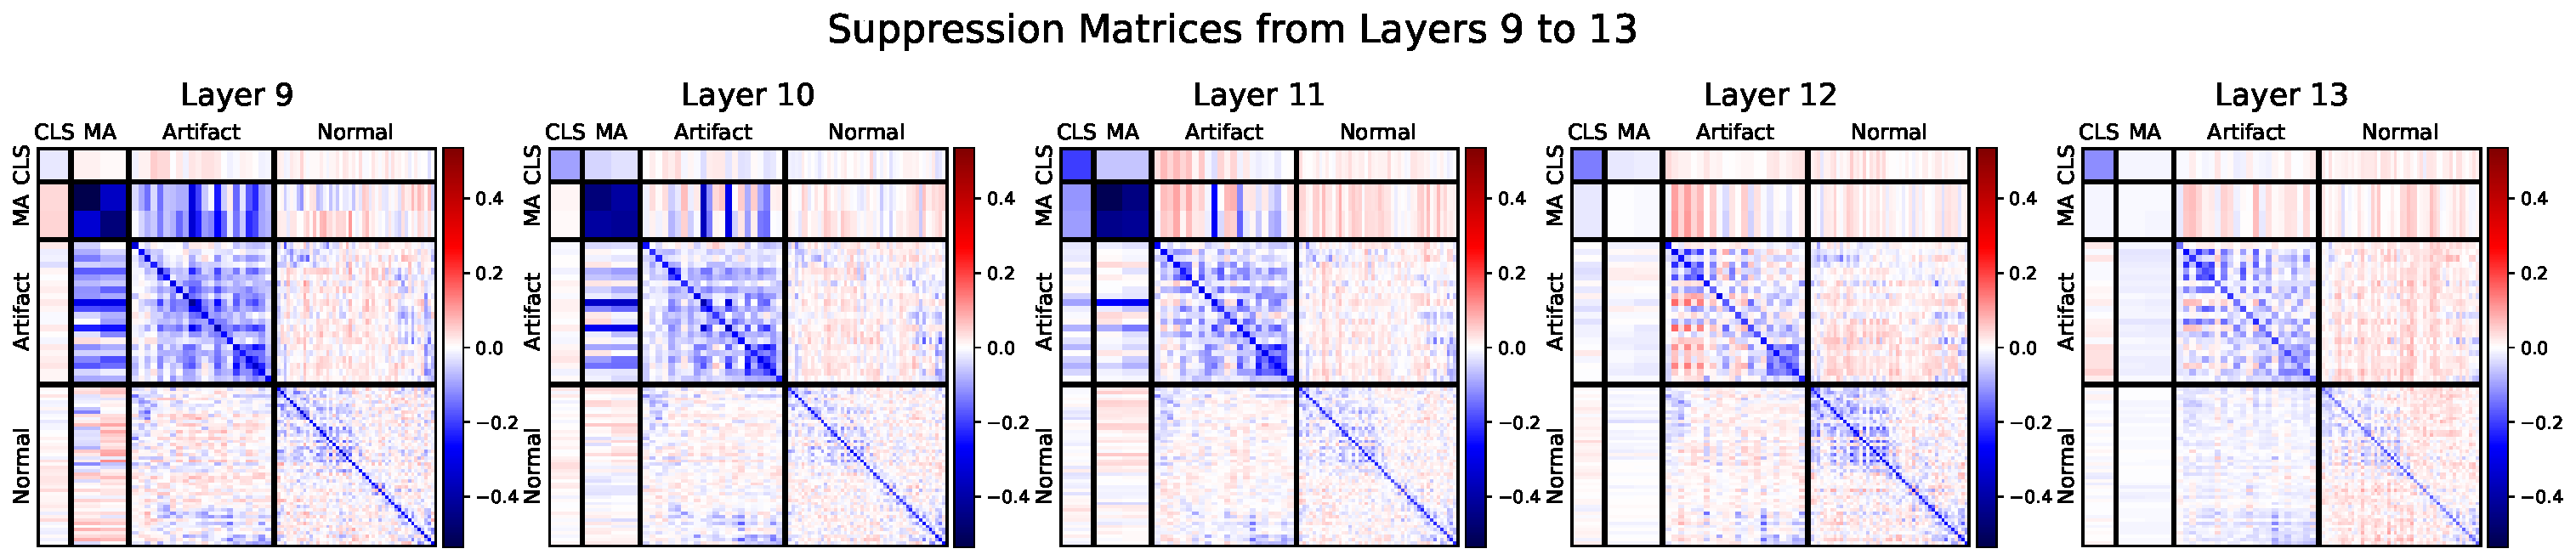
\includegraphics[width=1\linewidth]{figs/suppression_transition_L9toL13.pdf}
    \vspace{-1.5em}
    \caption{We observe in layers 9 and 10 that the pairwise suppression within the set of (potential) sink tokens is particularly strong. This effect decays and is absent at layers 12 and beyond. We also observe that the attention projection of the subspaces of massive tokens onto other tokens is particularly small after layer 12, which is consistent with findings that the values of massive tokens post-emergence are significantly smaller than average. It is also interesting to note that each token's projection onto itself is strongly negative, suggesting that its attention to itself may be partially destructive.}
    \label{fig:suppresion_transition}
\end{figure*}


\paragraph{Stabilization Phase (Layer 13+).}
Past layer 12, the suppression mechanism ceases while the massive tokens remain stably large, acting as bottlenecks for global information flow but no longer contending with other latent sink tokens.

\subsection{Implications for Efficient Attention}
% The structured hierarchy of token importance revealed by our analysis directly informs the design of Fast Nystr\"om Attention. By recognizing that:
% \begin{enumerate}
% \item CLS tokens provide global context
% \vspace{-0.2cm}
% \item Massive tokens dominate local attention patterns
% \vspace{-0.2cm}
% \item Artifact tokens represent latent redundancy
% \end{enumerate}

% we can strategically sample tokens for Nystr\"om approximation without compromising attention fidelity. The mutual suppression dynamics ensure that FPS naturally selects these critical tokens, as they occupy distinct regions of the feature manifold (Figure \ref{fig:dino_clip_artifacts}). 

The structured hierarchy of token importance revealed by our analysis—where (1) CLS tokens provide global context, (2) massive tokens dominate local attention patterns, and (3) artifact tokens represent latent redundancy—directly informs the design of Fast Nyström Attention. By recognizing these key roles, we can strategically sample tokens for Nyström approximation without compromising attention fidelity. The mutual suppression dynamics ensure that FPS naturally selects these critical tokens, as they occupy distinct regions of the feature manifold (Figure \ref{fig:dino_clip_artifacts}).


\subsection{Theoretical Underpinnings of Masking Gains}
Masking sink tokens in the later layers consistently boosts performance by rebalancing the attention dynamics toward more informative normal tokens. In tasks like classification or retrieval, the CLS token relies on attending to normal tokens for a rich global image representation. Sink tokens siphon attention from these normal tokens, degrading the CLS token’s ability to aggregate global information in the final layers. By masking sink tokens, we free the CLS token to attend more effectively to the meaningful patches, improving its final-layer representation. For segmentation or other dense tasks, we apply a linear probe to the final-layer patch embeddings. Sink tokens disrupt local coherence by overpowering normal tokens in attention. Masking preserves spatial fidelity yielding better dense predictions. While removing established massive tokens can trigger artifact tokens to grow, this process occurs earlier in the network. In the final layers, masking eliminates interfering activations without reintroducing new ones, denoising the final representation.




% Long version
% \section{Analysis of Sink Tokens}
% \label{sec:mechanisms}

% The efficiency and performance improvements demonstrated by our Fast Nystr\"om Attention (Section~\ref{sec:fna}) and masking-based denoising method (Section~\ref{sec:artifact_tokens}) stem from fundamental mechanisms governing token interactions in vision transformers. In particular, we identify \emph{mutual suppression} among tokens as the driving force behind the emergence of massive and artifact tokens. Below, we detail how this suppression shapes attention dynamics, underpins efficient approximations, and motivates our masking strategy.

% \subsection{Mechanisms of Token Suppression}

% Our experiments show that massive tokens emerge through a distinct \emph{phased} progression, driven by mutual suppression and magnified by MLP layers. Although the following layer indices refer specifically to CLIP ViT L-14, the same qualitative patterns arise in other large pretrained ViTs.

% \paragraph{Emergence Phase (Layers 9--10).}
% \begin{itemize}
% \item \textbf{Marginally Large Tokens.} In the early- to mid-layers (e.g., layers 9 and 10 in CLIP ViT L-14), tokens with slightly larger activations begin to exhibit suppressive behaviors toward other potential sink tokens (including themselves). 
% \item \textbf{Rich-get-Richer Effect.} These suppressive signals, when passed through the MLP’s nonlinear transformations, create a compounding feedback loop. Once a token has a slight size advantage, it increasingly dampens its competitors’ growth while continuing to grow itself.
% \end{itemize}

% Concretely, in a multi-head self-attention block, each token $j$ (serving as a \emph{key}) contributes a rank-$H$ subspace
% \begin{align}
%     \Sl{\ell}_j = \text{span}(\cbn{\Vl{\ell}_{h, j}}_{h \in [H]}) \subspace \R^d
% \end{align}
% which influences other tokens (as \emph{queries}) via the weighted combination
% \begin{align} \resizebox{\columnwidth}{!}{$
%     \attn{\ell}(\Embp{\ell})_i = \Olb{\ell} + \dss{j}{} \dss{h}{} \sf\pfrac{\Ql{\ell}_{h, i}{\mbf{K}^{(\ell)\top}_h}}{\sqrt{d'}}_j\Vl{\ell}_{h, j}{\mbf{O}^{(\ell)\top}_{h, weight}}.
% $}
% \end{align} 
% When a (potentially) massive token $j$ has a large norm, its subspace $\mathcal{S}_j^{(\ell)}$ tends to \emph{negatively} project onto other tokens in the MLP, yielding a \emph{destructive} or ``suppressive'' effect on their subsequent activations.

% \paragraph{Consolidation Phase (Layers 11--12).}
% \begin{itemize}
% \item \textbf{Attention Sinks.} The largest tokens fully mature into ``massive tokens'' around layers 11 and 12, absorbing a disproportionately large share of attention from all other tokens.
% \item \textbf{Destructive Interference.} Because attention weights are nonnegative (post-softmax), the dominant tokens effectively channel the MLP outputs in a way that \emph{further} suppresses remaining mid-sized contenders. Figure~\ref{fig:suppresion_transition} shows how these pairwise negative projections among massive tokens are strongest in mid-layers, explaining why incremental masking can reveal new ``artifact'' tokens.
% \end{itemize}

% Mathematically, if $P_{i,j}$ measures the mean normalized projection of token $j$’s subspace onto token $i$:
% \begin{align}
%     P_{i, j}
%     = \frac{1}{H} \dss{h}{} \frac{\innern{\emb{\ell}{i}, \Vl{\ell}_{h, j}}}{\normn{\emb{\ell}{i}}}
%     = \inner{\frac{\emb{\ell}{i}}{\normn{\emb{\ell}{i}}}, \frac{1}{H} \dss{h}{} \Vl{\ell}_{h, j}}
% \end{align}
% then a \emph{strongly negative} $P_{i,j}$ indicates $j$ significantly \emph{suppresses} $i$. In layers 9--10, the potential sink tokens heavily penalize each other’s growth; by layers 11--12, a small number of them have ``won'' the competition and become the new attention sinks.

% \begin{figure*}[t]
%     \centering
%     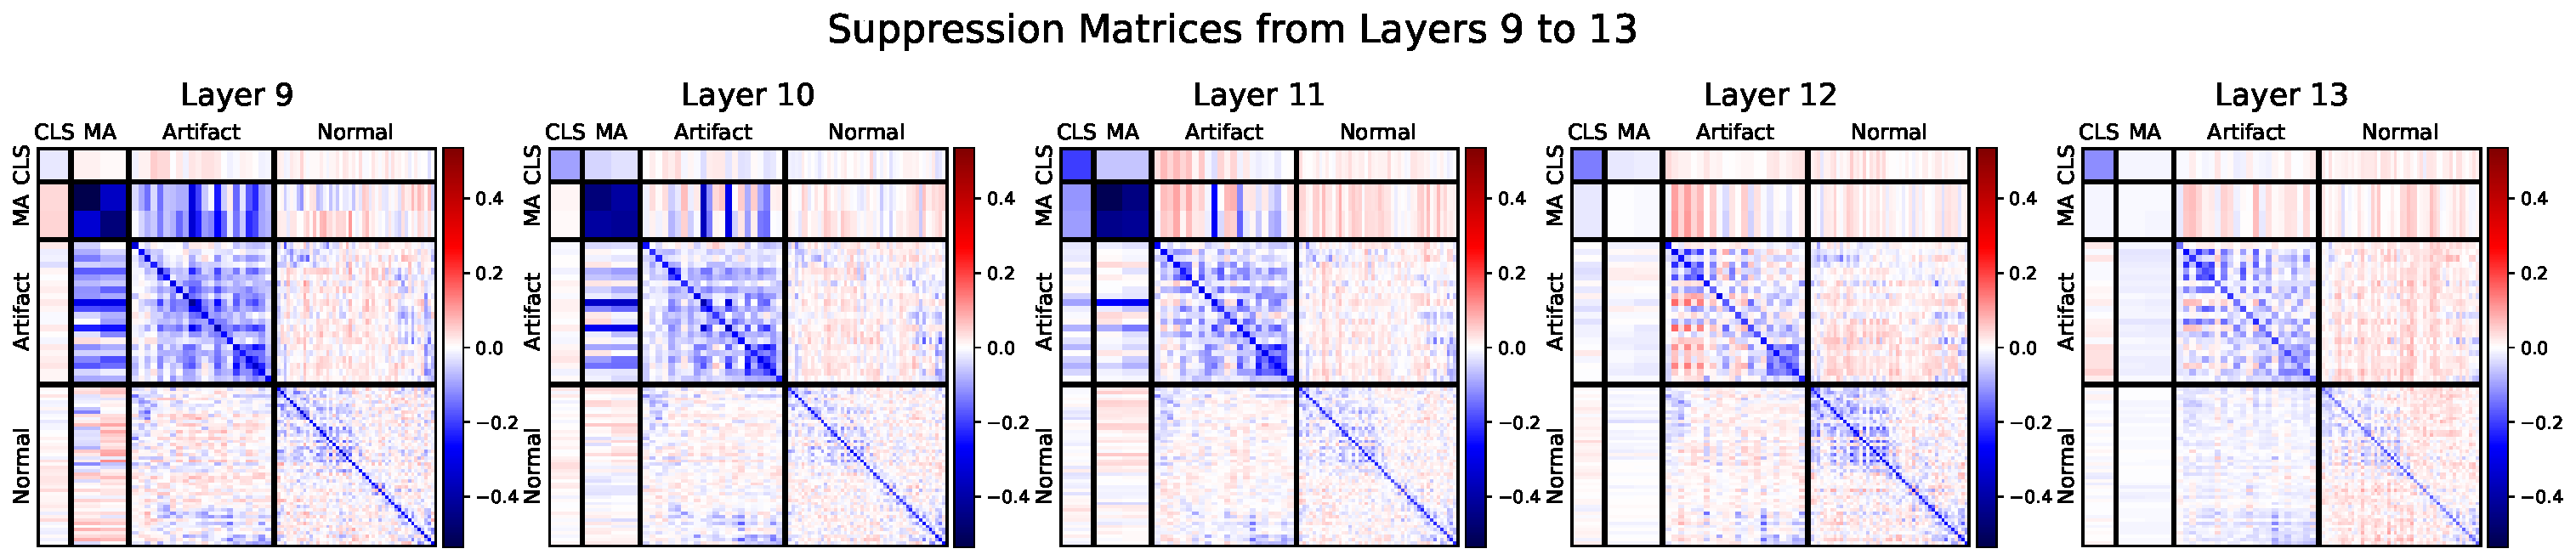
\includegraphics[width=1\linewidth]{figs/suppression_transition_L9toL13.pdf}
%     \caption{We can see in layers 9 and 10 that the pairwise suppression within the set of (potential) sink tokens is particularly strong which explains the behaviors we observe with different sinking patterns. This effect decays and is absent at layers 12 and beyond. We also observe that projection of the subspaces of massive tokens onto other tokens is particularly small after layer 12, which is consistent with findings that the values of massive tokens post-emergence are significantly smaller than average. It is also interesting to note that each token's projection onto itself is strongly negative, suggesting that its attention to itself may be partially destructive.}
%     \label{fig:suppresion_transition}
% \end{figure*}


% \paragraph{Stabilization Phase (Layer 13+).}
% \begin{itemize}
% \item \textbf{Persistent Bottlenecks.} Past layer 12, the suppression mechanism largely ceases. The massive tokens remain stably large, acting as bottlenecks for global information flow but no longer contending with other latent sink tokens.
% \item \textbf{Masking Outcomes.} Post-emergence masking of these massive tokens removes noise and improves feature quality (see Section~\ref{sec:performance_efficiency}). Because new sink tokens do not fully form at these later layers, the risk of overshadowing global or patch-level features is greatly diminished.
% \end{itemize}

% In summary, the mutual suppression mechanism becomes negligible after the model has solidified which tokens become massive. This explains why \emph{late-layer masking or denoising} consistently yields performance gains without risking a wholesale reconfiguration of the model's attention patterns.

% \subsection{Implications for Efficient Attention}
% The structured hierarchy of token importance revealed by our analysis directly informs the design of Fast Nystr\"om Attention. By recognizing that:
% \begin{enumerate}
% \item CLS tokens provide crucial global context
% \item Massive tokens dominate local attention patterns
% \item Artifact tokens represent latent redundancy
% \end{enumerate}

% we can strategically sample tokens for Nystr\"om approximation without compromising attention fidelity. The mutual suppression dynamics ensure that FPS naturally selects these critical tokens, as they occupy distinct regions of the feature manifold (Figure \ref{fig:dino_clip_artifacts}). 

% % Maybe since artifacts provide redudancy, not sampling MAs just causes artifacts to pick up the slack and performance doesn't drop by much

% \subsection{Theoretical Underpinnings of Masking Gains}
% Masking sink tokens (massive or artifact) in the later layers consistently boosts performance by rebalancing the attention dynamics toward more informative normal tokens. Specifically:

% \begin{itemize}
%     \item \textbf{Improving CLS Aggregation.}
%     In tasks like classification or retrieval, the CLS token relies on attending to normal tokens for a rich global image representation. Sink tokens siphon attention from these normal tokens, degrading the CLS token’s ability to aggregate global information. By masking sink tokens, we free the CLS token to attend more effectively to the meaningful patches, improving its final-layer representation.

%     \item \textbf{Enhancing Dense Outputs.}
%     For segmentation or other dense tasks, a linear probe is applied to the final-layer patch embeddings. Sink tokens disrupt local coherence by overpowering normal tokens in attention. Masking them preserves spatial fidelity and yields better dense predictions.

%     \item \textbf{Self-Limiting Interference.}
%     While removing established massive tokens can trigger artifact tokens to grow, this process occurs earlier in the network. In the final layers, masking eliminates interfering activations without reintroducing new ones, denoising the model’s final representation.
% \end{itemize} 






% \subsection{ORIGINAL ANALYSIS}


% We propose an explanation of the mechanisms involved in both forming and determining massive tokens that are consistent with all of several experiments comparing the behaviors under different masking conditions. Our claims are summarized in the following: \ref{sec:appendix_analysis} \begin{itemize}
%     \item The additive signal emitted by (potential) sink tokens are suppressive signals that reduce the magnitude of all other (potential) sink tokens including and particularly itself.

%     \item The largeness of a token lends to its suppressive signal, on one hand producing a compounding effect that makes marginally massive tokens in layer 9 particularly massive by layer 13, but on the other hand producing a reversal effect where secondary tokens that are allowed to grow unobstructed in turn suppress the primary massive tokens.

%     \item The largeness of a token lends to its attention sink \textit{viability}, which can be understood as its logit before the softmax. This largeness is both limited and determined by its facility to grow via layers 11 and 12 in absence of attention.

%     \item The suppression mechanism is no longer present after the formative layers of massive tokens, i.e. after layer 12. Any combination of masking or sinking thereafter has no impact on largeness or the distribution of attention amongst sink tokens.
% \end{itemize}

% Our in-depth analyses supporting those claims are provided in Appendix \ref{sec:appendix_analysis}. We can visualize the proposed suppression mechanism by examining the impact on each token in attending to another token. Specifically, consider the attention decomposition given in equation \ref{eqn:attn} where \begin{align} \resizebox{\columnwidth}{!}{$
%     \attn{\ell}(\Embp{\ell})_i = \Olb{\ell} + \dss{j}{} \dss{h}{} \sf\pfrac{\Ql{\ell}_{h, i}{\mbf{K}^{(\ell)\top}_h}}{\sqrt{d'}}_j\Vl{\ell}_{h, j}{\mbf{O}^{(\ell)\top}_{h, weight}}.
% $}
% \end{align} In effect, each token as a key provides some rank $H$ subspace \begin{align}
%     \Sl{\ell}_j = \text{span}(\cbn{\Vl{\ell}_{h, j}}_{h \in [H]}) \subspace \R^d
% \end{align} that is weighted in linear combination by the attention matrix to produce the attention output. Furthermore, we know the weights of the linear combination must be positive because the attention weights are bounded by $0$ and $1$. Therefore, for each query token $i$ and value token $j$, we can examine the projection of subspace $\Sl{\ell}_j$ onto input embedding $\emb{\ell}{i}$ to determine its signal, where a strongly negative projection indicates strong suppression. The mean pairwise projection can be computed as \begin{align}
%     P_{i, j}
%     = \frac{1}{H} \dss{h}{} \frac{\innern{\emb{\ell}{i}, \Vl{\ell}_{h, j}}}{\normn{\emb{\ell}{i}}}
%     = \inner{\frac{\emb{\ell}{i}}{\normn{\emb{\ell}{i}}}, \frac{1}{H} \dss{h}{} \Vl{\ell}_{h, j}}
% \end{align} and is shown in Figure \ref{fig:suppression_transition_layers}. We normalize the magnitude of the query token so that visualization of the per-token impact is not influenced by the discrepancy in sizes, but not by the size of the transmitting subspace as to maintain the relative impact of different tokens.


% \begin{figure*}[t]
%     \centering
%     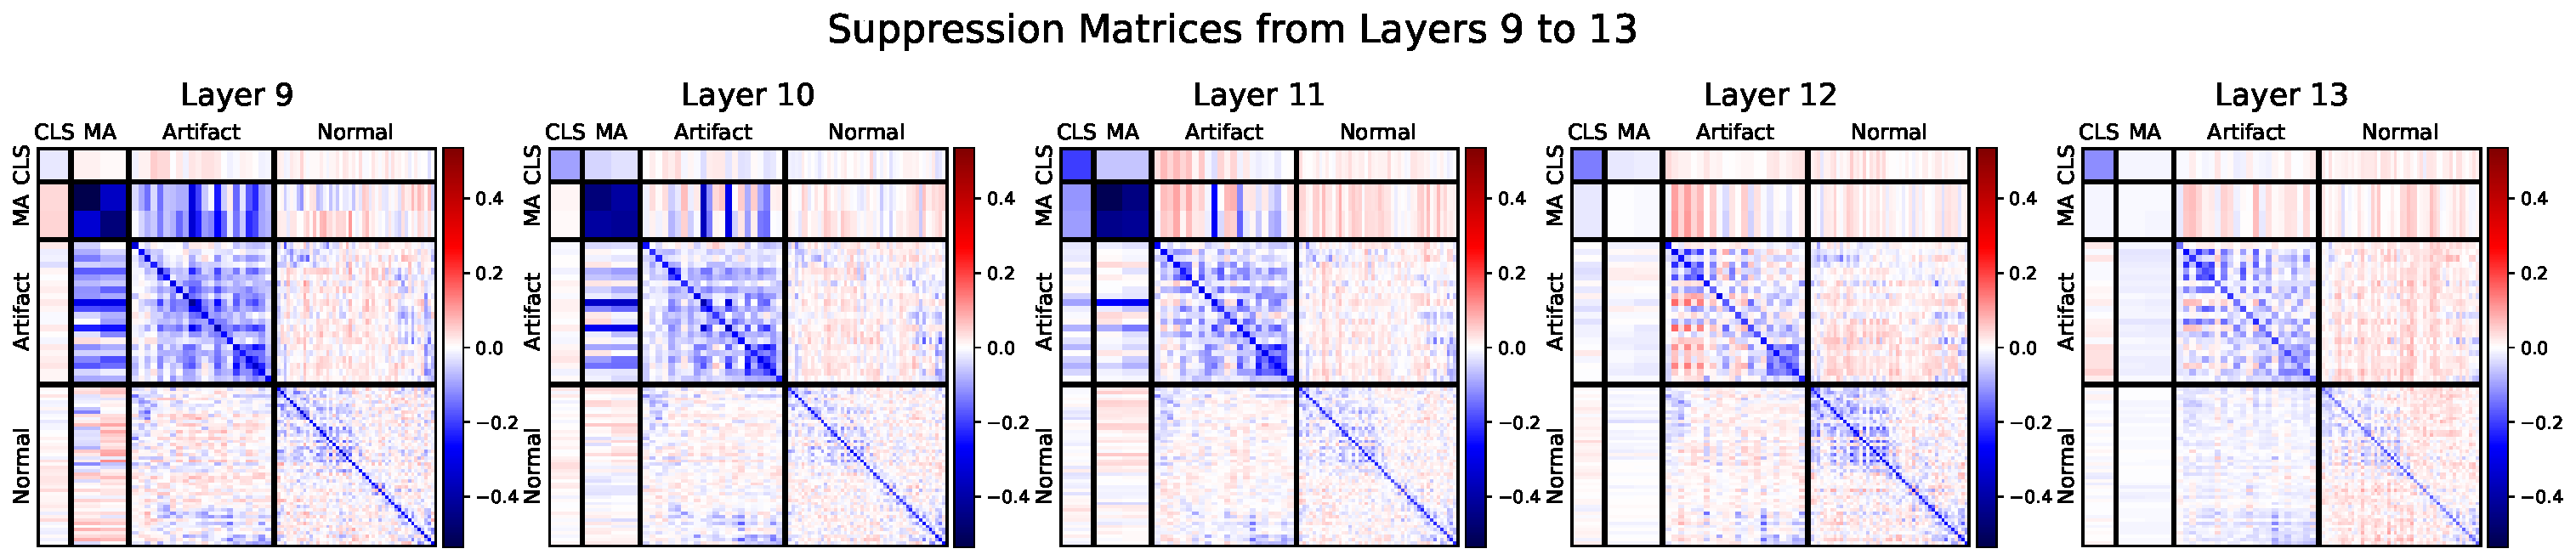
\includegraphics[width=1\linewidth]{figs/suppression_transition_L9toL13.pdf}
%     \caption{We can see in layers 9 and 10 that the pairwise suppression within the set of (potential) sink tokens is particularly strong which explains the behaviors we observe with different sinking patterns. This effect decays and is absent at layers 12 and beyond. We also observe that projection of the subspaces of massive tokens onto other tokens is particularly small after layer 12, which is consistent with findings that the values of massive tokens post-emergence are significantly smaller than average. It is also interesting to note that each token's projection onto itself is strongly negative, suggesting that its attention to itself may be partially destructive.}
%     \label{fig:suppression_transition_layers}
% \end{figure*}






